\section{Heat module - Part 2}
\subsection{Goal and Complexity}
\subsection*{Complexity: Beginner}

\subsection*{Prerequisites: Tutorial: heat module - part 2.}

The goal of this tutorial is to show further applicability of the $DRUtES$ heat module in 1D. We simulate heat conduction in a wall with two materials to understand the effects of layering of materials with different thermal properties.\medskip

\begin{figure}[!h]
\centering
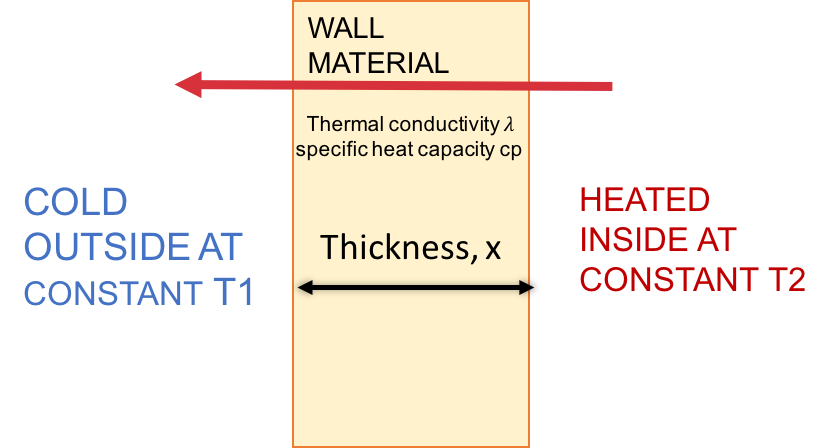
\includegraphics[width=8cm]{Fig_heat2/heat_cond_simple.png}
\end{figure}

Similar to tutorial 1, three configuration files will be modified step by step. All configuration files are located in the folder \emph{drutes.conf} and respective subfolders. \begin{enumerate}
\item For selection of the module, dimension and time information we require \emph{global.conf}.  \emph{global.conf} is located in \emph{drutes.conf / global.conf}. 
\item To define the mesh or spatial discretization in 1D,  we require \emph{drumesh1D.conf}. \emph{drumesh1D.conf} is located in \emph{drutes.conf / mesh / drumesh1D.conf}. 
\item To define heat conduction, we require \emph{heat.conf}. \emph{heat.conf} is located in \emph{drutes.conf / heat / heat.conf}. 
\end{enumerate}
$DRUtES$ works with configuration input file with the file extension .conf. Blank lines and lines starting with \# are ignored. The input mentioned in this tutorial therefore needs to be placed one line below the mentioned keyword, unless stated otherwise. 

\newpage
\subsection{Scenarios}

For all scenarios, we assume that the wall is between a heated room, which is maintaining a constant temperature of 20 $^{\circ}$C, and the outside world during winter, which for the sake of simplicity is at a constant temperature of 0 $^{\circ}$C.

\begin{table}[!h]\caption{\label{tab_heat}Material properties needed for scenarios.}
\adjustbox{max height=\dimexpr\textheight-5cm\relax,
           max width=\textwidth}{

\small\begin{tabular}{l c c c}
\hline
& specific heat capacity & density & thermal conductivity\\
& c$_p$ &  $\rho$ & $\lambda$ \\
Material & [J kg$^{-1}$ K$^{-1}$] & [kg m$^{-3}$] & [W m$^{-1}$ K$^{-1}$  ] \\
 \hline
Stone concrete & 750 & 1400 & 1.7 \\
Cotton &  1340& 1550 &0.04 \\
\hline
\end{tabular}
}
\end{table}


\section*{Scenario 1}

Heat conduction through a 20 cm wall. 15 cm are made of stone concrete and 5 cm are made of cotton fibre.

$global.conf$: Choose correct model, dimension, time discretization and observation times. This is the same as in heat tutorial 1.
\begin{enumerate}
\item Open \textbf{\emph{global.conf}} in a text editor of your choice. 
\item Model type: Your first input is the module. Input is \textbf{heat}.
\item Initial mesh configuration \begin{enumerate}
\item The dimension of our problem is 1. Input: 1.
\item We use the internal mesh generator. Input: 1. 
\end{enumerate}
\item Error criterion (not needed here, leave at default value) \begin{enumerate} 
\item Maximum number of iteration of the Picard method: 20 
\item h tolerance: 1e-2.
\end{enumerate}
\item Time information 
\begin{enumerate} 
%\item integration method is 3 point formula. Input: 30. 
\item Time units are in hours: input h
\item Initial time: 1e-3.
\item End time: 24.
\item Minimum time step: 1e-6.
\item Maximum time step: 0.1.
\end{enumerate}
\item Observation time settings \begin{enumerate}
\item Observation time method: 2
\item Set file format of observation: pure. Output in 1D is always in raw data. Different options will not impact output in 1D.
\item Make sequence of observation time: n
\item Number of observation times: 11
\item Observation time values: 2, 4, 6, 8, 10, 12 ,14 ,16, 18, 20, 22. Use a new line for each input. \textit{DRUtES} automatically generates output for the initial time and final time. DRUtES will generate 13 output files, e.g. \textit{heat\_temperature-x.dat}, where x is the number of the file and not the output time. The initial time is assigned an x value of 0. 
\end{enumerate}
\item Observation point settings \begin{enumerate}
\item Observation point coordinates: 0.0, 0.2. Use a new line for each input. \textit{DRUtES} will generate 2 output files, e.g. \textit{obspt\_heat-x.out}, where x is the ID of the observation point. 
\end{enumerate}
\item Ignore other settings for now. 
\item Save $global.conf$
\end{enumerate}


$drumesh1D.conf$: Mesh definition, i.e. number of materials and spatial discretization. Here is were the configuration files are different to heat tutorial one. 
\begin{enumerate}
\item Open \textbf{\emph{drumesh1D.conf}} in a text editor of your choice. 
\item Geometry information: 0.2 m - domain length
\item Amount of intervals: 1
\item
\adjustbox{max height=\dimexpr\textheight-5cm\relax,
           max width=\textwidth}{
\small\begin{tabular}{|c | c | c|}
\hline
density & bottom & top \\
 \hline
0.005 & 0 & 0.2 \\
\hline
\end{tabular}
}
\item Number of materials: 2
\item \adjustbox{max height=\dimexpr\textheight-5cm\relax,
           max width=\textwidth}{
\small\begin{tabular}{|c | c | c|}
\hline
id & bottom & top \\
 \hline
1& 0 & 0.15 \\
2 & 0.15 &0.2 \\
\hline
\end{tabular}
}
\end{enumerate}

\emph{heat.conf}: Heat module after Sophocleous (1979). 
Here, it is important to make sure everything is defined for 2 layers. 2 lines of input are required, even when the input is identical. 

\begin{enumerate}
\item Open \emph{heat.conf} in a text editor of your choice. 
\item Couple with Richards equation: n
\item Number of materials or layers: 2
\item Specific heat capacity of the wall material: 
Material 1 is stone concrete: \\750 J kg$^{-1}$ K$^{-1}$ x 1400 kg m$^{-3}$ = 1.05E6 J m$^{-3}$ K$^{-1}$ = $\frac{1.05E6~\mathrm{W~s~m^{-3}~K^{-1}}}{3600~\mathrm{s~h^{-1}}}$ \\= 291 W h m$^{-3}$ K$^{-1}$. \\
Material 2 is cotton fibre: \\1340 J kg$^{-1}$ K$^{-1}$ x 1550 kg m$^{-3}$ = 2.08E6 J m$^{-3}$ K$^{-1}$ = $\frac{2.08E6~\mathrm{W~s~m^{-3}~K^{-1}}}{3600~\mathrm{s~h^{-1}}}$ \\= 576 W h m$^{-3}$ K$^{-1}$. 
\item Specific heat capacity of liquid: 0 (for both materials)
\item Anisotropy: There is no anisotropy. The value is 0 (for both materials)
\item Heat conductivity of the wall material: \\ Material 1: 1.7 W m$^{-1}$ K$^{-1}$ \\ Material 2: 0.04 W m$^{-1}$ K$^{-1}$
\item There is NO heat convection of water: 0 (for both materials)
\item The initial temperature is 0$^{\circ}$C across the entire domain: 0 (for both materials)
\item There is no heat source: 0 (for both materials)
\item This is identical to heat tutorial 1. We have 2 boundaries at both ends of the wall. We assume a constant temperature of 0$^{\circ}$C outside. We assume the inside is heated and the temperature maintained at exactly 20$^{\circ}$C. We therefore know the temperature at the boundaries. We also know that these values do not change in time. They can be describes as time-constant Dirichlet boundary conditions. \\
\adjustbox{max height=\dimexpr\textheight-5cm\relax,
           max width=\textwidth}{
\small\begin{tabular}{|c | c | c| c|}
\hline
boundary id & boundary type & use bc.dat & value \\
 \hline
101& 1 & n & 20.0 \\
102& 1 & n & 0.0 \\
\hline
\end{tabular}
}

\item Save heat.conf.
\end{enumerate}

\section*{Run scenario 1}
Run the simulation in the terminal console.
\begin{enumerate}
\item Make sure you are in the right directory. 
\item To execute $DRUtES$: \\
\$ bin/drutes
\item After the simulation finishes, to generate png plots execute provided R script: \\
\$ Rscript drutes.conf/heat/heatplots.R concretecotton1
\item The output of the simulation can be found in the folder out

\end{enumerate}

\section*{Tasks for scenario 1}

\begin{enumerate}
\item Describe the temperature distribution. How long does it take for the temperature distribution to become linear between the two observation points?
\item How large is the steady state heat flux through the wall?
\item Let's assume a wall area of A=15 m$^2$. Use the observation point at the boundary between the wall and the inside of room. How large was the cumulated heat loss 24 h. How much will be lost after 48 h when the set-up does not change?
\end{enumerate}


\section*{Result of scenario 1}

\subsection*{Question 1}
Figure \ref{plot1} shows two distinct linear temperature distributions. The temperature distributions appears to have not changed significantly over the last observation times indicating a steady state. A 5 cm thick cotton fibre wall is between the concrete stone and the heated inside. The overall heat flux at the inside border is therefore quite low as the input of heat has to travel through badly conducting material first. 

\begin{figure}[!h]
\centering
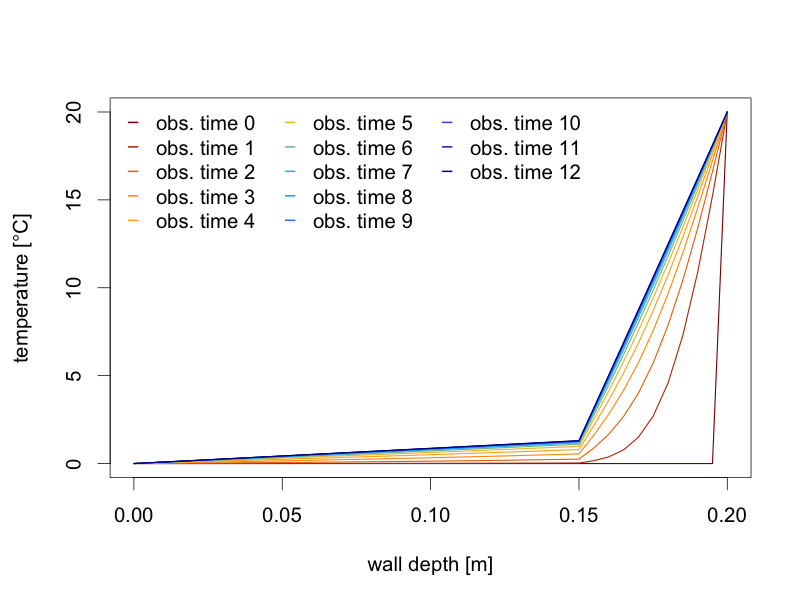
\includegraphics[width=10.5cm]{Fig_heat2/obs_time_temp_concretecotton1.png}
\caption{\label{plot1}Plot of observation times for a wall with a 15 cm outer stone concrete layer and an inner 5 cm cotton fibre layer  generated with Rscript heatplots.R}
\end{figure}

\subsection*{Question 2}

\begin{figure}[!h]
\centering
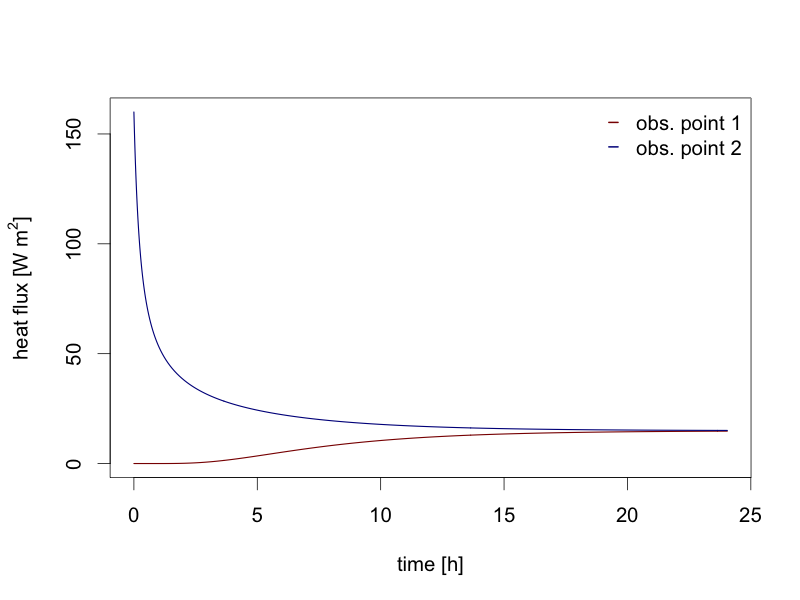
\includegraphics[width=10.5cm]{Fig_heat2/obs_point_temp_concretecotton1.png}
\caption{\label{plot2} Heat flux at observation points 1 and 2 for a wall with a 15 cm outer stone concrete layer and an inner 5 cm cotton fibre layer generated with Rscript heatplots.R}
\end{figure}

Looking at the raw data, it appears that steady-state has not actually been reached, but that the change in heat flux is becoming slower and is converging towards 15 W m$^{-2}$. 

\newpage
\subsection*{Question 3}

Figure \ref{plot3} shows the cumulative heat flux in observation points 1 and 2, both ends of the wall. The cumulative heat flux after 24 h at observation point is 538 W m$^{-2}$. With a wall area of 15 m$^2$ this results in $Q = 538~\mathrm{W~h~m^{-2}}\cdot~15~\mathrm{m^{2}}= 8070 ~\mathrm{W~h}$. 
For the next 24 h, the heat flux will be constant at 15 $\mathrm{~W~m^{-2}}$. The total heat loss will therefore be $Q=15 \mathrm{~W~m^{-2}}~\cdot 24~\mathrm{h}~\cdot~15~\mathrm{m^{2}}=5400 \mathrm{~W~h}$.

\begin{figure}[!h]
\centering
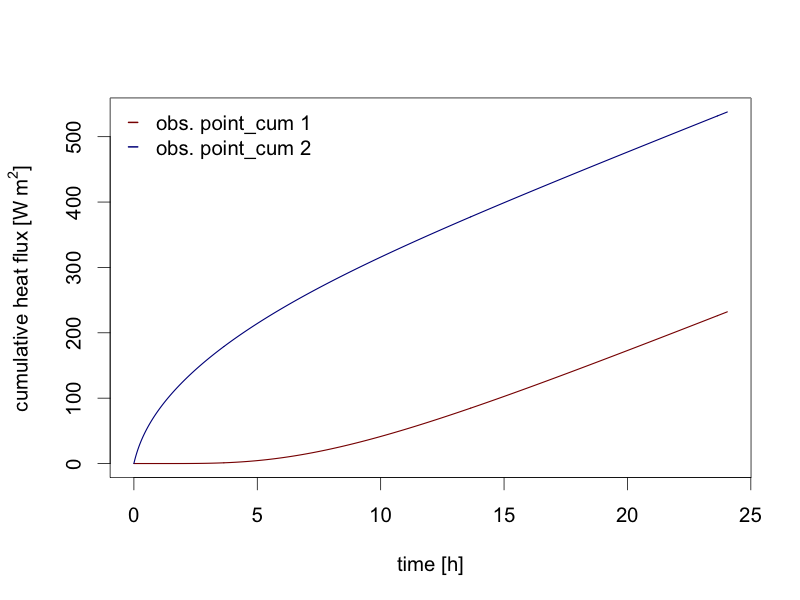
\includegraphics[width=10.5cm]{Fig_heat2/obs_point_cum_temp_concretecotton1.png}
\caption{\label{plot3} Cumulated heat flux at observation points 1 and 2 for a wall with a 15 cm outer stone concrete layer and an inner 5 cm cotton fibre layer generated with Rscript heatplots.R}
\end{figure}

\newpage

\section*{Scenario 2}

\begin{enumerate}
\item Open \emph{heat.conf} in a text editor of your choice. 
\item Swap the order of materials for specific heat capacity and thermal conductivity. Now, the the outer wall layer is made of cotton fibre and the inner layer is made of concrete.
\item Save heat.conf.
\end{enumerate}

\section*{Run scenario 2}
Run the simulation in the terminal console.
\begin{enumerate}
\item Make sure you are in the right directory. 
\item To execute $DRUtES$: \\
\$ bin/drutes
\item After the simulation finishes, to generate png plots execute provided R script: \\
\$ Rscript drutes.conf/heat/heatplots.R cottonconcrete
\item The output of the simulation can be found in the folder out

\end{enumerate}

\section*{Tasks for scenario 2}

\begin{enumerate}
\item Answer the same questions as for scenario 1. What is different?
\end{enumerate}

\section*{Result of scenario 2}
\subsection*{Question 1}
Figure \ref{plot4} shows the inner concrete layer becomes linear quite quickly, but that the outer cotton fibre layer has not reached linearity after 24 h. Also taking Fig. \ref{plot5} 
\begin{figure}[!h]
\centering
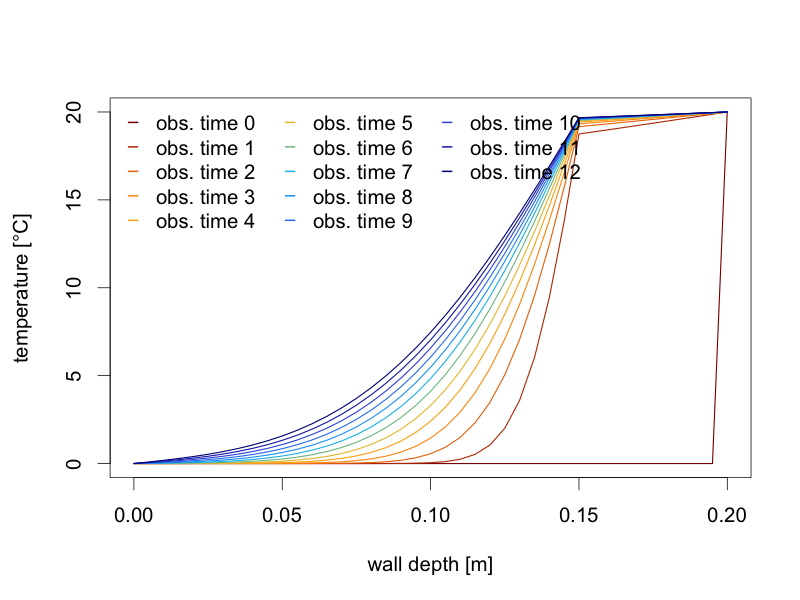
\includegraphics[width=10.5cm]{Fig_heat2/obs_time_temp_concretecotton2.png}
\caption{\label{plot4}Plot of observation times for a wall with a 15 cm thick outer cotton layer and a 5 cm inner concrete stone layer generated with Rscript heatplots.R}
\end{figure}

\subsection*{Question 2}

The system has not reached a constant heat flux, but the heat flux will be between 0.7 and 111 W m$^{-2}$. A long simulation (not shown) of 240 h shows that the steady state hea flux converges towards 53 W m$^{-2}$.

\begin{figure}[!h]
\centering
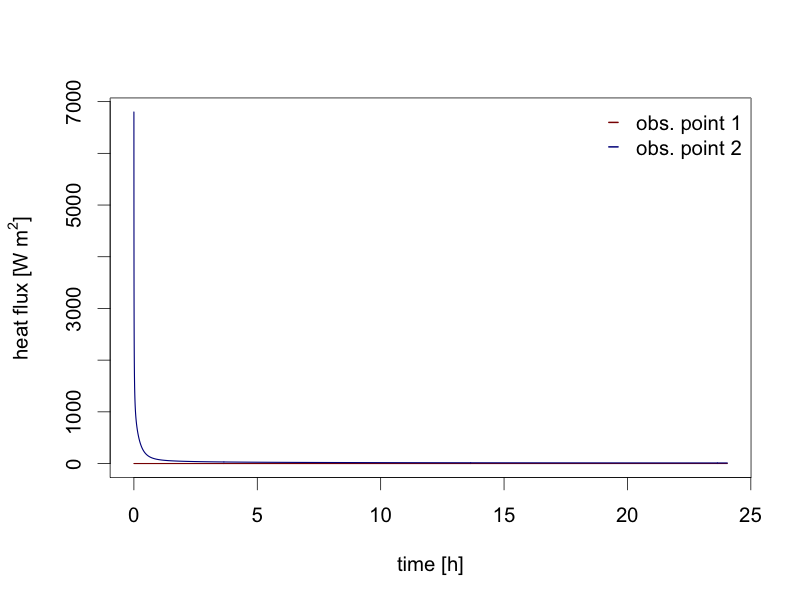
\includegraphics[width=10.5cm]{Fig_heat2/obs_point_temp_concretecotton2.png}
\caption{\label{plot5} Heat flux at observation points for a wall with a 15 cm thick outer cotton layer and a 5 cm inner concrete stone layer generated with Rscript heatplots.R}
\end{figure}


\subsection*{Question 3}

The cumulative heat flux after 24 h at the inner boundary is higher than in scenario 1, namely 797 W m$^{-2}$. With a wall area of 15 m$^2$ this results in $Q = 797~\mathrm{W~h~m^{-2}}\cdot~15~\mathrm{m^{2}}= 11955 ~\mathrm{W~h}$. 
For the next 24 h, the heat flux will not be constant and needs to be numerically simulated. 

\begin{figure}[!h]
\centering
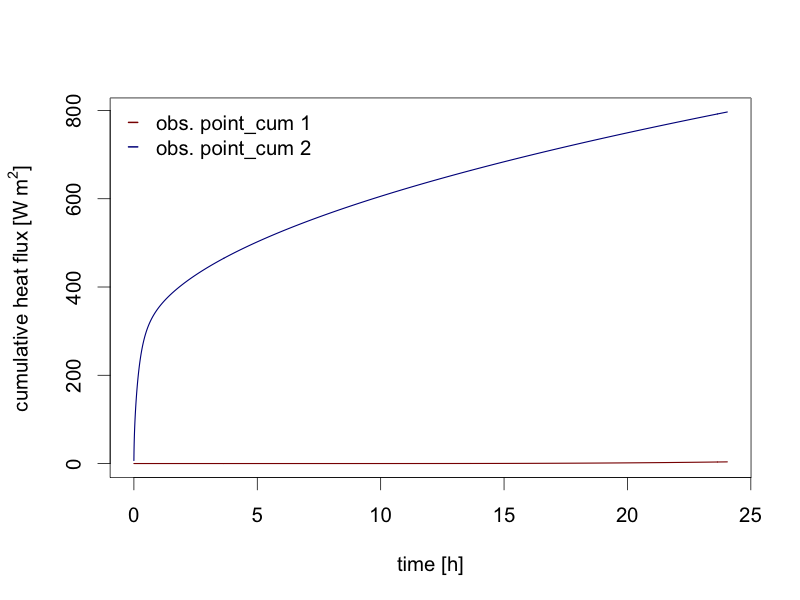
\includegraphics[width=10.5cm]{Fig_heat2/obs_point_cum_temp_concretecotton2.png}
\caption{\label{plot6} Cumulated heat flux at observation points for a wall with a 15 cm thick outer cotton layer and a 5 cm inner concrete stone layer generated with Rscript heatplots.R}
\end{figure}

\newpage
\newpage
\newpage

\subsection{Outcome}
\begin{enumerate}
\item You got familiar with the $DRUtES$ heat module in 1D with 2 layers.
\item You simulated heat conduction through a wall with layered materials.
\item You understand the effects of layering of materials with different heat capacities and thermal conductivities.
\item You understand how layering affects when a system is in \emph{steady state}.
\end{enumerate}
--